\documentclass[border=3mm]{standalone}
\usepackage{tikz}
\usetikzlibrary{calc}
\begin{document}
	\centering
	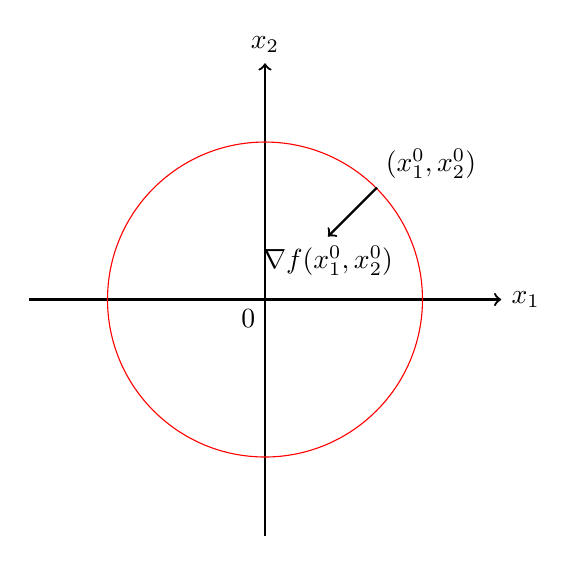
\begin{tikzpicture}
		\coordinate (O) at (0,0);
		\coordinate (V) at (1.41,1.41);
		\coordinate (G) at (0.8,0.8);
		\draw[->,thick] (-3,0)--(3,0) node[right]{$x_1$};
		\draw[->,thick] (0,-3)--(0,3) node[above]{$x_2$};
		\draw (O) node [below left]{$0$};
		\draw [red] (O) circle (2cm) ;
		\foreach \i in {45}{
			\draw [<-,thick] (0.8,0.8) --++ (\i:0.88cm)coordinate(p\i){};
			%\draw ($(p\i)!1!-90:(2,2)$) -- ($(p\i)!1!90:(2,2)$);
		}
		\draw (V) node [above right ]{$(x_1^0,x_2^0)$};
		\draw (G) node [below  ] {$\nabla f(x_1^0,x_2^0)$};

		
	\end{tikzpicture}
\end{document}